\documentclass[a4paper, 12pt]{article}
\usepackage[T1]{fontenc}
\usepackage[utf8]{inputenc}
\usepackage{lmodern}
\usepackage[english]{babel}
\usepackage{amsmath}
\usepackage{amsfonts}
\usepackage{amssymb}
\usepackage{relsize}
%\usepackage{abraces,mathtools}
%\usepackage[hidelinks,hyperfootnotes=false]{hyperref}
\usepackage{empheq}
\usepackage{graphicx}
\usepackage{parskip}
\usepackage{indentfirst}
\usepackage[font={small, it}]{caption}
\usepackage[coverpage]{polytechnique}
\usepackage{booktabs}
\usepackage{multirow}

\title{Specificity and constraints in Peptide-Protein bindings in the mouse proteome}
\subtitle{Report for 3rd Year Research Project}
\author{Dhruv SHARMA}
%\usepackage{geometry}

\newcommand*\widefbox[1]{\fbox{\hspace{2em}#1\hspace{2em}}}
\begin{document}
\pagebreak
\maketitle
\tableofcontents
\pagebreak
\part{Introduction}
	This report details the work done towards the fulfillment of the requirements of the department of Physics at Ecole Polytechnique. I undertook this research project under the guidance of Dr. Remi Monasson at the Laboratoire de Physique Theorique at the Ecole Normale Superieure in Paris.

	\indent
	The aim of the project was to study the interactions between short peptide chains and a specific section of signaling proteins called PDZ Domains. One of the aspects that we study here is the specificities of interactions between peptides and PDZ domains. It is well known that macromolecules such as proteins and enzymes interact in a specific manner with other macromolecules and biomolecules. What interested us over the course of the study are the constraints present in the peptide sequences due to the specificity of their interactions with PDZ domains. We will also have an occasion to understand similar constraints on the PDZ domain sequences. 

	This report is organized as follows. After a brief introduction to the biological importance of PDZ Domains, we explain the experiments performed by \textbf{Insert reference here}. Using these experiments, Stifler et al created a model which is capable of predicting whether a peptide will bind to a PDZ domain given the sequence of the peptide. We shall explain the data that Stifler et al have provided. The first two models that we propose utilise the data provided by Stifler et al. 

	Once the data presented and the biological context established, we present a first model which seeks to understand the constraints imposed on the peptide sequences under the effect of mutations. We present the results derived from this model and discuss the limitations. A second improved model is then proposed which considers error rates as probabilities. We present some interesting observations on the basis of this model. In particular, we show how certain positions are particularly constrained over all peptides and present a simple way of the calculating the level of constraint. 

	Finally, to render the study of peptide-PDZ domain specificity complete, we explain how we could integrate the PDZ Domain sequences into the modeling. This is done by a regression method called the \textit{Lasso}. We shall have the chance to present the lasso method in more detail in the relevant section. 

	We conclude with a summary of our findings and possible directions of further improvements. 

	\section{PDZ Domains}

	Let us begin by explaining PDZ Domains, their importance, their structure and how they bind to other macromolecules. PDZ domains are short sections of proteins composed of 80-90 amino acids. PDZ Domains are usually found in signaling proteins where they regulate processes such as the separation of cell membranes. PDZ itself is an acronym for the first three letters of three proteins: Post-synaptic density protein (PSD95), Drosophilia disc large tumor suppressor (Dlg1) and zonula occludens-1 protein (zo-1)

	PDZ Domains are usually composed of 80-90 amino acids and many PDZ domains can be present within a single protein. Multiple domains within the same protein can have similar functions or different functions, each of which will bing to a different part of the target protein or a different protein altogether.

	PDZ Domains always bind to the C-terminal of certain specific sections of the target proteins. The binding occurs within a binding pocket formed by the domain. The binding pocket are usually formed by the first 20 amino acids. A diagram showing the positions of the binding pocket as well as the target peptide are shown below. 

	\begin{figure}
	\label{PDZ_Positions}
	\centering
	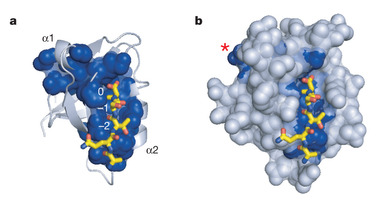
\includegraphics[width=10cm]{Images/pdz.jpg}
	\caption{\textbf{Left}: We show the PDZ domain (in blue) with the target peptide (yellow). The C-terminal of the target peptide is numbered 0 whilst the preceding amino acids are numbered in descending order. 
	\textbf{Right}: The position of the PDZ-Domain within the parent protein is shown. The position marked with a little star shows that during the binding process there are other parts of the PDZ domain which are involved and not just the binding pocket}
	\end{figure}	

	\section{Explanation of the data of Stifler et al}

	Now that we have given a small introduction to PDZ domains we shall explain the work done by Stifler and co-authors which we sought to extend and improve upon.

	The article that we have considered is titled "PDZ domain binding specificity is optimized across the mouse proteome". In this article, Michael Stifler and co-authors sought to characterize the selectivity between 157 PDZ domains and 217 target peptides found in the mouse proteome. To this end, they created a model which could predict whether a given PDZ domain would bind to a target peptide given the sequence of the target peptide.

	In their model, the last 5 positions near the C-terminal of the target peptide are considered. The model can be summarized in the following simple equation: 

	\begin{align}
	\label{model_base}
	\phi_{i} = \sum_{p,q} A_{p,q} \theta_{i,p,q} > \tau_{i}
	\end{align}

	where for a given PDZ Domain $i$, we can calculate a binding score $\phi_{i}$. $A$ is an indicator of the peptide sequence : $A_{p,q} =1$ if the amino acid at position $p$ of the peptide is $q$ and $A_{p,q} =0$ otherwise. The numbers $\theta_{i,p,q}$ are the parameters that need to be fit to the experimental data. $\tau_{i}$ is a scoring threshold which is different for each domain $i$. The values $\theta_{i,p,q}$ are to be interpreted in the following fashion: $\theta_{i,p,q} > 0$ if the PDZ Domain $i$ prefers amino acid $q$ at position $p$ more than the other PDZ domains, negative if it prefers it less, and 0 if it has no bias relative to the other domains. $\tau_{i}$ is defined as the $m$th percentile of the $\phi_{i}$'s for all the peptides in the model that bound to the domain $i$. To make predictions using this model, it suffices to know the sequence of the target peptide and compute $\phi_{i} - \tau_{i}$ for the domain $i$. If the domain binds with the target protein then this number is positive and negative otherwise. 

	The data used to fit the model was obtained by protein micro-array assays. Each PDZ Domain-peptide pair under consideration was verified for binding during the experiment. The researchers were able to model 74 domains among the 157 domains experimented upon. The experimental results of these experiments are available to us in the form of an interaction matrix which tells us whether a PDZ domain $i$ binds to a target peptide $j$ or not. 

	For each of the 74 domains successfully modeled, we also possess the parameters $\theta_{i,p,q}$ allowing us to test the model on newer peptide sequences. We also possess the error rates for the model. These are given in terms of false positive and false negative rates. These error rates interpreted as empirical probabilities were used in one of the models presented later in the report.

	\section{Questions asked and answered}

	With the biological context established and the various data that we possess explained, let us now briefly the discuss the questions that we sought to answer over the course of the project. 

	Firstly, we sought to understand the effect of mutations on the specificity of domain-peptide interactions. It is well known that PDZ domains bind to only certain specific target peptides and not to others. What if the target peptide suffered a point mutation? Will the PDZ domain still bind to the peptide? 

	A related question concerns the level of constraint imposed on the peptides due to the specificity of their interactions with PDZ domains. If the peptide were to suffer a point mutation and if it continued to bind to the PDZ domain, it then becomes interesting to consider the extent to which the peptide can undergo mutations before it stops binding to the peptide. Inversely, if the peptide doesn't accept many mutations, it is again interesting to analyze whether there are certain positions or amino acids which impose constraints on the sequence. 

	All such questions were modeled, analyzed and understood in this project.

\pagebreak
\part{First Model}
	\section{Features of the model}

	Our first model sought to study the effects of the introduction of mutations in the target peptide sequences conserving all the while the interaction matrix. The mutations considered were point mutations whereby one amino acid at a particular position was muted into another one. To this end, we define a parameter $\alpha$ which corresponds to binding or non-binding for the domain-peptide pair in the interaction matrix, $\alpha=1$ if PDZ domain $i$ binds to peptide $j$ and $\alpha = -1$ otherwise. Since we want to introduce mutations that conserve the interaction matrix, we begin with the natural sequence of a given peptide and introduce mutations in the natural sequence. 

	Now, we start from a natural sequence of the peptide $l$. Once a point mutation has been introduced in the sequence, we calculate the binding score $\phi$ for this new sequence using \eqref{model_base}. We then define a probability of binding and non-binding in the following manner:

	\begin{align}
	\label{model_1_naive}
	p(\alpha_{i,l}=1) & = \frac{1}{1+e^{-\phi}} \\
	p(\alpha_{i,l}=-1) & = \frac{1}{1+e^{\phi}}
	\end{align}

	for the domain $i$ and peptide $l$. Here we continue to use the label $l$ for the peptide even though the \emph{new} binding score $\phi$ is calculated for a mutated sequence and not the natural sequence for the peptide $l$

	Furthermore, we define an \emph{energy} for each peptide $l$ as:

	\begin{equation}
	\label{model_1_energy}
	\mathrm{E} = \sum_{i} \mathrm{log}(1+e^{-\alpha_{i,l}\phi_{i,l}})
	\end{equation}

	where the sum is over all domains $i$ in our data set. The energy defined can thus be defined for any sequence derived by introducing point mutations into the base sequence of the peptide $l$. In practice, we have a natural sequence, we then introduce a mutation into the sequence, calculate the probabilities $p(\alpha=1)$ or $p(\alpha=-1)$ for a given domain $i$ and sum the natural logs of these probabilities over all the 74 domains. 

	Once the mutations have been introduced and an energy defined for a new sequence derived from some natural peptide sequence, we now need a method to determine whether we accept or reject these mutations. To this end, we adopt the Metropolis algorithm, used for performing Monte Carlo simulations. The choice of performing a Monte Carlo simulation is a natural one since the sequence space consists of $20^5$ sequences and rather than sampling the whole space uniformly, it is more economical to perform a Monte Carlo (hereby MC) simulation.

	The general flow of the simulations was as follows:

	\begin{enumerate}
	\item 
	We begin with a single peptide and introduce point mutations starting with the natural sequence of the peptide. 
	\item 
	We then compare the energies, as defined in \eqref{model_1_energy}, between two sequences $\mathrm{E}_{old}$ and $\mathrm{E}_{new}$. 
	\item 
	We then use the Boltzmann factor to attribute probabilities to each of the energies  $\mathrm{E}_{old}$ and $\mathrm{E}_{new}$, where the boltzmann factor is 
	\begin{align}
	\label{boltz}
	p(E) \propto e^{-\beta E}
	\end{align}

	where $\beta$ is called the inverse temperature and the factor of proportionality is the partition function. Since we will take ratios of probabilities, we need not compute the partition function explicitly. 

	\item 
	We define the acceptance probability as :

	\begin{align}
	\label{prob_acceptance}
	p_{\mathrm{accept}} = \mathrm(min(1, \frac{p_{new}}{p_{old}}))
	\end{align}

	where $p_{new}$ and $p_{old}$ are computed using the Boltzmann factor.

	\item 

	Given $u \in U[0,1]$ where $U[0,1]$ is the uniform probability distribution, the new sequence is accepted if $ u < p_{\mathrm{accept}}$
	\end{enumerate}

	We chose the value of $\beta=1$. We performed 10 cycles of Monte Carlo runs, whereby during each run we affected 1000 mutations to each of the 217 peptides in our data set. 

 	\section{Results}

 	The first quantity that we computed was the initial distribution of energies i.e. energies computed for each of the peptides using only their natural sequences. 

 	\begin{figure}
 	\label{hist_ini_energies}
 	\centering
 	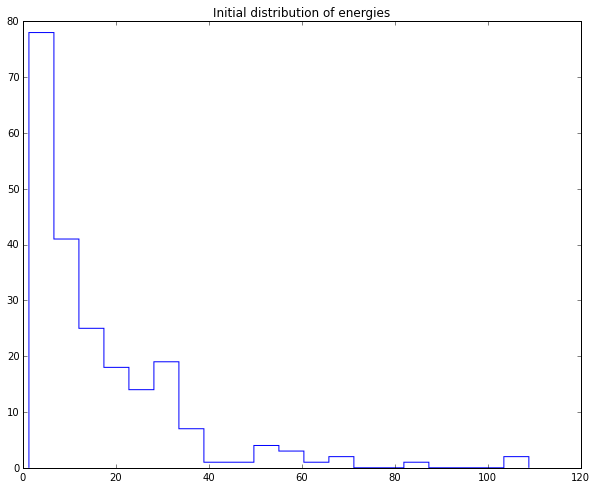
\includegraphics[width=8cm]{Images/hist_ini_energies.png}
 	\caption{The distribution of initial energies of the peptides. We observe that the energies are well spread out, with the majority in the range from 0-5 and the maximum energy close to 100}
 	\end{figure}

 	We compare this distribution to the distribution of energies of those sequences which were accepted during the Monte Carlo runs

 	\begin{figure}[!h]
 	\label{hist_final_energies} 
 	\centering
 	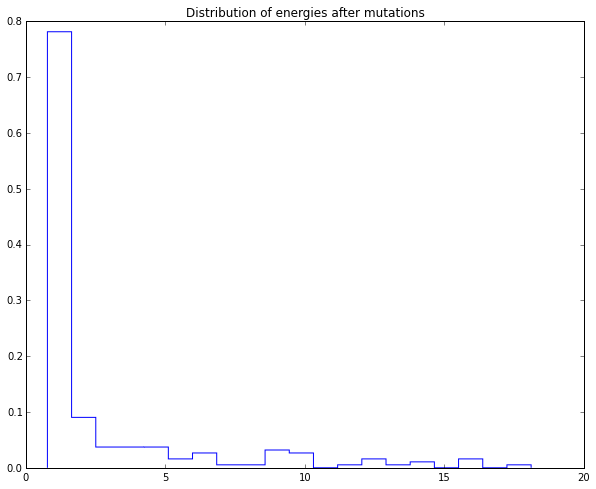
\includegraphics[width=8cm]{Images/hist_fin_energies.png}
 	\caption{Here the spread is reduced. The maximum is close to 19.}
 	\end{figure} 

 	We see a reduction by a factor of 5 in the spread of energies before and after the Monte Carlo runs.

 	The next quantity that we considered was the probability of having a given amino acid at any position for any peptide. To this end, we computed the frequency matrix which tells us how often a given amino acid was accepted during the Monte Carlo runs. 

 	\begin{figure}[!h]
 	\label{freq_matrix}
 	\centering
 	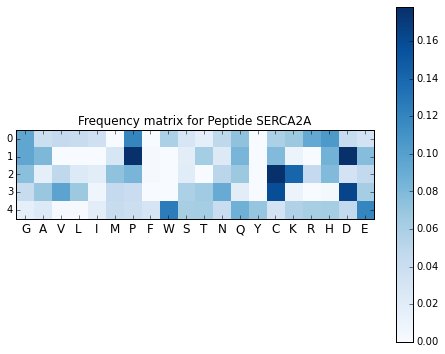
\includegraphics[width=7cm]{Images/freq_matrix.png}
 	\caption{The frequency matrix gives a very simple and visual way of deciding whether a given peptide is susceptible of undergoing mutations.} 
 	\end{figure}

 	Here the peptide considered \textbf{SERCA2A} has the sequence \textbf{PAILE}. We observe that the most frequent amino acid during the MC runs was Proline(P) and not Alanine (A). Thus we can already see that this peptide is susceptible to undergo mutations. This claim is further supported with the spread over all the 20 amino acids. 

 	The peptide \textbf{Cftr} presents a rather particular case for us. Its frequency matrix is presented here. We remark very clearly how, except for the last position, the other positions are not susceptible at all to undergo mutations. Even the mutations that do occur in the last position are not drastic. The natural sequence of \textbf{Cftr} is \textbf{QETRL}. On the last position, we see that the only mutation accepted is a transformation from Leucine (L) to Isoleucine, which would not be sterically important. Thus we find an interesting case of the existence of strong constraints on the sequence of the peptides in the face of mutations. During the MC runs, \textbf{Cftr} oscillates between two sequences: natural sequence \textbf{QETRL} and a mutated sequence \textbf{QETRI} 

 	\begin{figure}
 	\label{cft_freq}
 	\centering
 	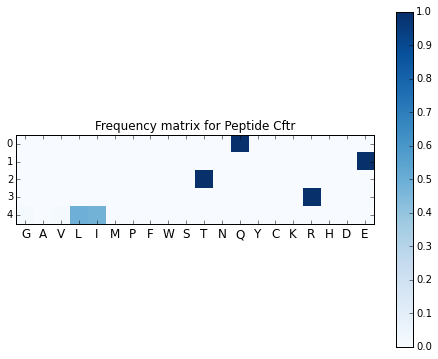
\includegraphics[width = 7cm]{Images/cftr.png}
 	\caption{The sequence for \textbf{Cftr} is very strictly constrained accepting mutations only at the last position.}
 	\end{figure} 

 	\section{Limitations}

 	This model however is not without its limitations. Another particular case that we consider is the peptide \textbf{APC} which has the natural sequence \textbf{LVTSV} and has a natural energy of 108. When we consider the evolution of the energy over the course of any one MC cycle, we observe that it has a tendency to very quickly reduce its energy as is evident from the plot below

 	\begin{figure}[!h]
 	\label{apc_evol}
 	\centering
 	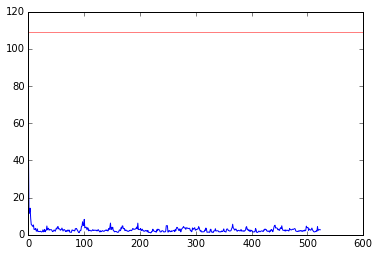
\includegraphics[width=7cm]{Images/apc_evol.png} 
 	\caption{The evolution of the energies of the mutated sequences of \textbf{APC} during one MC cycle. Out of 1000 mutations possible, it accepts close to 530 mutations, showing a great susceptibility to undergo mutations. Red line shows the natural energy.}
 	\end{figure} 

 	This behavior is related to the particular nature of the peptide \textbf{APC} as well as the errors inherent in the model. We ascribe this behavior to the erroneous predictions of the model which needs to be accounted for in a newer model. This is the subject of the next section. 
\pagebreak
\part{Improvements over first model: Bayesian Modeling}
	
	The case of the peptide \textbf{APC} tells us that we cannot consider all the predictions of the model to be true and we need a way to integrate the error rates which are present in any predictive model. To this end, we propose a refined model based on conditional probabilities.
\section{Error rates as probabilities}
	Any predictive model is seldom 100\% perfect and there are always cases where the predictions of the model are in contradiction with the experimental facts. This is the case with the model used by Stifler et al. The information concerning the error rates for their model is known to us and thus we can integrate this extra information to refine our model. 

	To do this, we need to understand the error rates that we possess. These error rates are reported as true positive rate, false positive rate, true negative and false negative rates. To be more precise, considering that the model predicts binary values 0(False) or 1(True):

	\begin{enumerate}
	\item 
	\textbf{True Positive Rate (TP)}: $\frac{\text{Number of events predicted to be True}}{\text{Number of events actually True}}$
	\item 
	\textbf{True Negative Rate (TN)}: $\frac{\text{Number of events predicted to be False}}{\text{Number of events actually False}}$
	\item 
	\textbf{False Positive Rate(FP)}: $\frac{\text{Number of events predicted to be True}}{\text{Number of events actually False}}$
	\item 
	\textbf{False Negative Rate(FN)}: $\frac{\text{Number of events predicted to be False}}{\text{Number of events actually True}}$
	\end{enumerate}

	For the model proposed by Stifler, these values are given as:

\begin{table}[]
\centering
\caption{Error rates from Stifler et al.}
\label{tab_error_rate}
\begin{tabular}{@{}ll@{}}
\toprule
Error Rate & Value \\ \midrule
TP         & 96\%  \\
FN         & 4\%   \\
FP         & 15\%  \\
TN         & 85\%  \\ \bottomrule
\end{tabular}
\end{table}

The way these error rates are defined reminds us of the definition of conditional probabilities. And thus, we can interpret these error rates as conditional probabilities. If the model makes a prediction on a new piece of data, these rates then tell us with what probability the experimental value was +1 or -1. Thus we have, 
\begin{align}
\label{inter_cond}
\text{TP} &= \mathbb{P}(\text{Model} = 1 | \text{Experiment} = 1) \\
\text{FN} &= \mathbb{P}(\text{Model} = -1 | \text{Experiment} = 1) \\
\text{FP} &= \mathbb{P}(\text{Model} = 1 | \text{Experiment} = -1) \\
\text{TN} &= \mathbb{P}(\text{Model} = -1 | \text{Experiment} = -1)
\end{align}

We can then recast Table~\ref{tab_error_rate} in the following manner:

\begin{table}[!h]
\centering
\caption{Error rates as conditional probabilities}
\label{tab_proba_error}
\begin{tabular}{@{}ccc@{}}
\toprule
Model & Exp & P(Model|Exp) \\ \midrule
+1    & +1  & 0.96         \\
-1    & +1  & 0.04         \\
+1    & -1  & 0.15         \\
-1    & -1  & 0.85         \\ \bottomrule
\end{tabular}
\end{table}

\section{Updated Bayesian model}

Having cast error rates as probabilities we can now use Bayes rule to invert the Table~\ref{tab_proba_error} i.e. calculate the probability $\mathbb{P}(\text{Exp|Model})$. This can be done using the following equation:

\begin{align}
\label{invert_proba_bayes}
\mathbb{P}(\text{Exp|Model}) = \frac{\mathbb{P}(\text{Model|Exp}) \mathbb{P}(\text{Exp})}{\mathbb{P}(\text{Model})}
\end{align}

where $\mathbb{P}(\text{Model})$ is a normalising factor that needs to be calculated from the experimental data and $\mathbb{P}(\text{Exp}=1)$is for a given peptide, number of domains that it binds to, and similarly for $\mathbb{P}(\text{Exp}=-1)$. We can thus calculate a the \textit{posterior} probabilities for each peptide: by using the interaction matrix for calculating $\mathbb{P}(\text{Exp})$, with $\mathbb{P}(\text{Model})$ is calculated by normalising the probability $\mathbb{P}(\text{Exp|Model})$. 

We can create a posterior probability matrix for the complete data set, by summing over all the peptides in the data set. We thus have

\begin{table}[!h]
\centering
\label{tab_proba_posterior}
\caption{Posterior Probability Matrix}
\begin{tabular}{@{}ccc@{}}
\toprule
Exp & Model & P(Exp|Model) \\ \midrule
+1  & +1    & 0.1818       \\
-1  & +1    & 0.8181       \\
+1  & -1    & 0.0016       \\
-1  & -1    & 0.9983       \\ \bottomrule

\end{tabular}
\end{table}

We observe that the value $\mathbb{P}(\text{Exp=1|Model=1})$ is very small. This is because for the whole data set $\mathbb{P}(\text{Exp=1})$ is very small $\sim$ 0.03. 

For the purposes of introducing mutated sequences into the model, we would now like to compute the probability of binding (non-binding) given a mutated sequence. To this end, we use the chain rule to get the following expression for $\mathbb{P}(\text{Exp|Sequence})$:

\begin{align}
\label{proba_model_chain}
\mathbb{P}(\text{Exp|Sequence}) = \sum_{\text{Model}=\pm 1} \mathbb{P}(\text{Exp|Model}) \mathbb{P}(\text{Model|Sequence})
\end{align}

where 
\begin{equation}
\mathbb{P}(\text{Model|Sequence}) = \frac{1}{1+e^{-\textrm{y}_{\text{model}} \phi}}
\end{equation}
and where $\textrm{y}_{\text{model}} = \pm 1$ are the values predicted by the model (+1 for binding and -1 for non-binding) and $\phi$  is the score calculated from \eqref{model_base}. We once again compute an energy for each peptide, this time for the updated probability \eqref{proba_model_chain}. Using the variable $y$ for the values that Exp and Model can take, we write the energy for the peptide $l$ as :

\begin{align} 
\label{energy_bayes}
\mathrm{E} = - \sum_{i} \mathrm{log}(\mathbb{P}(y^{i,l}_{\text{Exp}} | \text{seq}))
\end{align}

where the sum runs over all the domains $i$. Using this redefined energy, we perform MC simulations with the same parameters as before.

\section{Results}

\begin{enumerate}
\item 
We first compare the distribution of energies in the updated model. In the updated model, the spread of energies is limited between 0 and 20. More importantly, the distribution of energies once the mutations have been affected is similar. We thus see already a great improvement in the model whereby we have prevented drastic drops in energy like the one we saw in the case of \textbf{APC} 

\begin{figure}[!h]
\label{update_model_energy}
\centering
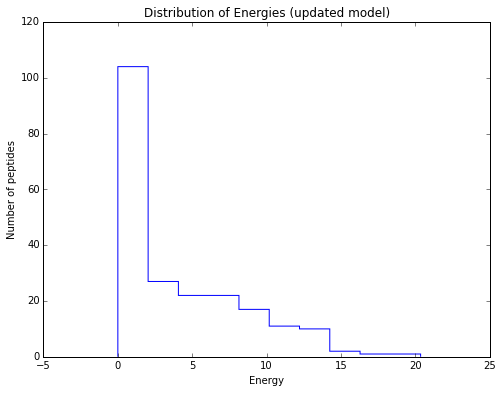
\includegraphics[width=10cm]{Images/update_model_dist.png}
\end{figure}

\item 

This time we had more confidence in the model with respect to the previous one, we computed other relevant quantities that could give us information about the constraints present in the sequences of the peptides. One of the first quantities that we computed was the entropy of the peptide from the frequency matrix. We define the entropy of the peptide $l$ for the position $k$ in its sequence as :

\begin{equation}
\label{entropy_definition}
S^{l}_{k} = -\sum_{a=1}^{a=20} p_{k,a} \mathrm{log}(p_{k,a})
\end{equation}

where the sum $a$ runs over all the 20 amino acids and $p_{k,a}$ is the probability of finding amino acid $a$ at position $k$. This probability can readily be computed from the frequency matrix for the peptide $l$. The entropy is a particularly relevant quantity since it provides a direct way of determining the degree of constraint that is present in the position $k$ for any peptide. In particular, a value of $S=0$ tells us that the peptide doesn't accept any mutations on the position considered and is thus highly constrained. 

Furthermore, we can also compute the quantity $S^{l} = \sum_k S^{l}_{k}$ which is the sum of the entropies over all positions for the peptide l. This quantity tells us how much liberty we do have while performing mutations of the natural peptide sequence. To facilitate our understanding and provide a simple way of distinguishing between different types of peptides, we divide all the 217 peptides based on a quantity called the binding number $\mathrm{bn}$, which is just the number of domains that a peptide binds to. 

As a first indication of the dependence of the behavior of peptides as a function of their binding number, we trace the number $S^l$. 

\begin{figure}
\label{sum_entropy_bn}
\centering 
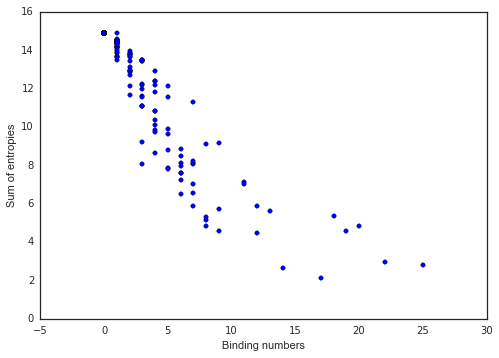
\includegraphics[width=7cm]{Images/sum_vs_bn.png}
\caption{Dependence between entropy and binding number}
\end{figure} 

We remark that the entropy varies inversely with an increase in binding number. This shows that higher the binding number, higher are the constraints present over the natural sequence of the peptide. Thus, we are led to a closer analysis of the position wise entropies $S^{l}_{k}$for different values of the binding number. 

\item 
We know that if $S^{l}_{k}=0$ for any position $k$ then it implies that the position $k$ is immune to mutations. After dividing the peptides by their binding numbers, we searched for any peptides which showed such behavior. Remarkably and contrary to what we would have believed initially, such peptides are present over a large range of binding numbers: we would accept that a peptide with bn=25 would have some position constrained owing to its extremely low entropy value. However, we also observed constraints for binding numbers as low as bn=3. The peptide with bn=3 showing such a behavior is \textbf{NMDAR2C}

\begin{figure}[!h]
\label{bn_3_freq_matrix}
\centering
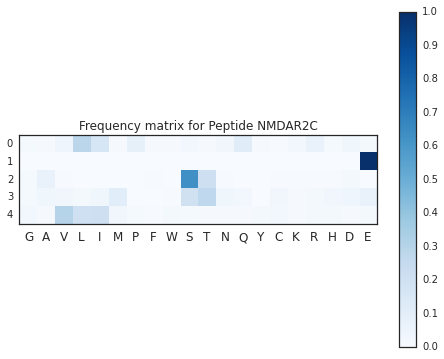
\includegraphics[width=7cm]{Images/nmdar2c.png}
\caption{The 2nd position in the sequence of \textbf{NMDAR2C} is clearly constrained. Even for other positions we see that the space of possible mutations isn't spread out over many amino acids.}
\end{figure}

\item 

After having observed the presence of constraints, we wanted to see whether any non-trivial correlations existed between the two positions. To determine which two positions could be potentially correlated, we computed the mutual information matrix, defined as follows:

\begin{equation}
\label{mi_definition}
\mathrm{MI}_{i,j} = \sum_{a=0, b=0}^{a=20, b=20} p_{i=a, j=b} \mathrm{log}(\frac{p_{i=a,j=b}}{p_{i,a} p_{j,b}})
\end{equation}

where $p_{i=a,j=b}$ is the joint probability of finding the amino acids $a$ and $b$ at positions $i$ and $j$ respectively and $p_{i,a}$ is the probability of finding amino acid $a$ at position $i$. The mutual information intuitively tells us how much information is considered in the variable X about the variable Y. In our case, by computing the mutual information matrix, we would be able to determine the correlated positions in the peptide sequence. 

\begin{figure}
\centering 
\label{mi_nmdar2c}
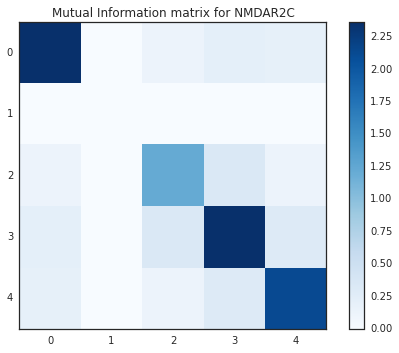
\includegraphics[width=7cm]{Images/nmdar2c_mi.png}
\caption{The mutual information matrix for NMDAR2C. The second position (1 in the figure) being completely constrained is not correlated with any of the other positions.}
\end{figure} 

The constraint on the position numbered 1 in the figure (the numbering used in the figures starts with 0, common in programming languages) is manifest in the mutual information matrix as well. It is completely independent of the other positions, implying that it is completely uncorrelated with any other position as well. This is just another way of saying that the position numbered 1 must conserve the amino acid found in the natural sequence irrespective of the other positions. 

From the mutual information matrix, we see that positions numbered 2 and 3 might be correlated. However, the computed correlations are very small, suggesting that the positions are only weakly correlated. This trend was observed for other peptides with different bn's as well. 

\begin{figure}
\centering 
\label{corr_2_3_nmdar2c}
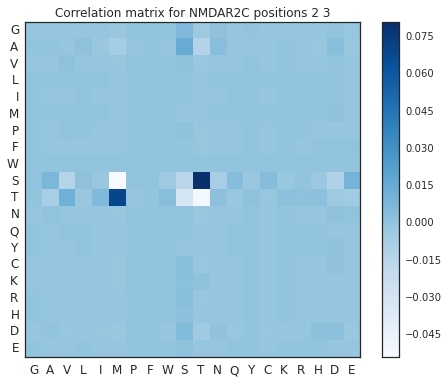
\includegraphics[width=7cm]{Images/nmdar2c_corr_2_3.png}
\caption{The normalized correlation coefficient matrix for correlations between the different pairs of amino acids. Barring a few amino acids, most amino acids are completely uncorrelated.}
\end{figure} 

\item 

From the frequency matrix we can compute the most probable sequence. This sequence is constructed by computing the amino acid with the highest probability of occurrence at any given position. We present here the most probable sequences for each of the 18 peptides which showed highly constrained behavior during the MC runs. 

\begin{table}[!h]
\centering
\caption{Peptides with constrained positions}
\label{Zero_entopy peptides}
\begin{tabular}{lllll}
\hline
Name       & MPS   & Base Sequence & Hamming Distance & Binding Number \\ \hline
           &       &               &                  &                \\ \hline
Caspr2     & KRWIC & KEWLI         & 3                & 5.0            \\ \hline
Cftr       & QETRL & QETRL         & 0                & 17.0           \\ \hline
Cnksr2     & LETHV & IETHV         & 1                & 25.0           \\ \hline
CRIPT      & KQTSV & KQTSV         & 0                & 12.0           \\ \hline
ctransprtr & NATRL & NATRL         & 0                & 8.0            \\ \hline
Nav1.      & RESNV & RESIV         & 1                & 9.0            \\ \hline
NMDAR2B    & IESDV & IESDV         & 0                & 8.0            \\ \hline
PKC        & LQAAV & LQSAV         & 1                & 8.0            \\ \hline
PMCA1      & IETSL & LETSL         & 1                & 19.0           \\ \hline
Sapk3      & LETAL & KETAL         & 1                & 20.0           \\ \hline
SSTR2      & ILAWV & IIAWV         & 1                & 22.0           \\ \hline
TAZ        & FLTWL & FLTWL         & 0                & 18.0           \\ \hline
TRPC4      & NHTRL & VTTRL         & 2                & 6.0            \\ \hline
NMDAR2C    & LESTV & LESEV         & 1                & 3.0            \\ \hline
Kv1.5      & RETDQ & RETDL         & 1                & 7.0            \\ \hline
Kv1.7      & MVTTV & MVTEV         & 1                & 13.0           \\ \hline
TRPM6      & NHTRL & DHTRL         & 1                & 5.0            \\ \hline
TRPV3      & PETSV & PETSV         & 0                & 12.0           \\ \hline
\end{tabular}
\end{table}

\item 

An interesting observation that we made during the search for the presence of constraints was that the last position, i.e. C-terminal amino acid was never constrained. This is surprising because PDZ domains bind to the C-terminal of the target peptides. The lowest values for the entropy and thus the most constraints were seen for positions numbered 2 and 3 in the diagrams, which would corresponds to -3 and -2 in the sequence of the peptide. No constraints were found for last position that is -4 either. 

\item 

Finally, we attempted to see whether by the removal of one PDZ domain would change the behavior of the peptides or not. It was found that it did not. However, on average the peptides accepted more mutations that with the presence of the domain. But these mutations were energetically unfavorable. 
\end{enumerate}

\textbf{Some Caveats}

\begin{enumerate} 
\item 
The peptide sequences considered here are made up only 5 amino acids. Thus, our modeling is necessarily local in nature and we are not aware of the relevant steric and chemical effects that might influence the binding between peptides and PDZ-domains. Furthermore, we know that the binding pocket is not the only part of the PDZ domain which is implicated in the binding, other positions far away from the binding pocket are involved too. Thus, by considering only those sections of the target molecules which are present near the binding pocket, our analysis can only be limited. 

\item 
There are many peptides for whom we didn't see any constraints whatsoever. This however should not mean that constraints are completely absent from these peptides. Far from it, this serves as a reminder of the limited scope of our study. With only 74 domains to play with, we cannot generalize the behavior of the peptides that we studied. 

\end{enumerate}

\pagebreak
\part{Integrating PDZ Domain sequences} 

After having studied the peptides present in our data set, we sought to integrate the sequences of the PDZ domains. We wanted to be able to propose a model using the sequences of the PDZ Domains which would be able to recreate the parameters $\theta_{i,p,q}$ of the original model \eqref{model_base}. To this end, we decided to use a simple linear model. However, this linear model is necessarily under-constrained. For instance if we consider one domain $i$, and we assume that we will consider only the first 20 amino acids in the sequence, it gives us a possible 400 parameters (20 amino acids $\times$ 20 positions) parameters to fit for 100 unknown variables. (For each domain $i$, we have 100 values for $\theta_{i,p,q}$: 5 positions on the peptide $\times$ 20 amino acids). An ordinary least squares regression would not be very efficient. However, the method \textbf{LASSO} or Least Absolute Shrinkage and Selection Operator is best adapted to our needs. This is the method that we decided to finally use. 
\section{The LASSO}

The LASSO is a method which forces the sum of the absolute value of the regression coefficients to be less than a fixed value, leading to certain regression coefficients to be set to zero. The condition of forcing the absolute sum of the coefficients to be less than a certain limit is known as \textbf{L1 Regularization}. 

The Lasso can be written as an optimization problem set in the form: 

\begin{equation} 
\label{lasso_eq_basic_form}
\min_{\beta_0, \beta}\left\{ \frac{1}{N} \sum_{i=1}^N (y_i-\beta_0 - X \beta)^2 \right\}  \text{ subject to } \sum_{j=1}^{p} \|\beta_j\| \leq t
\end{equation}

However, we can recast this equation in the Lagrangian form as follows:

\begin{equation}
\label{lasso_lagrange}
\min_{ \beta \in \mathbb{R}^p } \left\{ \frac{1}{N} \left\| y - X \beta \right\|_2^2 + \lambda \| \beta \|_1 \right\}
\end{equation}. 

Here, $y$ is the output of the model and $X$ is the data. In our case, the output variables are the $\theta_{i,p,q}$ for each of the domains $i$ and the $X$ correspond to a matrix of dimensions $n \times 20$ where $n$ is the length of the PDZ domain sequence that we consider. The matrix $X$ is defined as follows: $X_{n,a} = 1$ if the amino acid $a$ is at position $n$ and $X_{n,a} = 0$ otherwise. 

For a practical implementation, we considered 70 domains for whom we could find the complete sequence. For each of the domains the $\theta_{i,p,q}$ were collapsed into a vector of dimensions $100 \times 1$, and the $X^{i}$ were collapsed into a vector of size $ (n \times 20) \times 1$. Thus, the output variable $y$ had dimensions $70 \times 100$ while $X$ had dimensions $70 \times (n\times 20)$. The lasso was finally implemented with the open source library scikit-learn in Python. 

\section{Results}

We studied two configurations for the 
\part{Conclusion}

\end{document}